\section{Information Preservation}\label{sec:info}

\paragraph{Frozen probes overstate the loss.} A logistic truth probe fitted on original activations and applied
unchanged to SAE reconstructions loses 0.28--0.29 AUROC on GoT (Table~\ref{tab:m2}, Figure~\ref{fig:m2}). Earlier
versions of this project read this as truth information being lost. Adding isotropic noise with the same norm as the
SAE error causes almost the same drop (0.25--0.26), and a simpler mass-mean reader loses only 0.02--0.03. Most of the
frozen-probe collapse is therefore sensitivity of that reader to any perturbation of this size, not SAE-specific loss.

\paragraph{A smaller, real loss remains.} Readers re-trained on the reconstructions are 0.07--0.12 AUROC worse than
readers trained on the original activations for GoT, and 0.14--0.18 worse for the persona task. Re-training never
recovers the original performance, so no cell is classified as ``readout shifted''; no cell is ``preserved''. The
task label can be decoded from the reconstruction error alone (AUROC 0.62--0.77), so the lost information is still in
the activation, outside the SAE's reconstruction.

\paragraph{SAEs are never better than PCA.} At the same OWT reconstruction error, PCA keeps at least as much task
information as the SAE in every cell; the SAE is significantly worse in 52 of 81 GoT cells, 59 of 99 persona cells
and 81 of 90 neutral cells (one-sided paired bootstrap, BH-corrected).

\paragraph{Persona versus generic change.} Part of the persona loss is generic one-word-change information: the
re-trained gap is 0.07--0.13 larger for persona than for neutral swaps at layers 3--8, and about equal at layers 10--11.

\paragraph{Architecture differences are confounded.} On truth, ReLU loses least and JumpReLU most, the reverse of
the reconstruction ranking; on persona, ReLU loses most. Because task-level L0 is not matched, we do not interpret
these differences as architecture effects until E1 is run.

% generated by scripts/shared/build_paper_artifacts.py from results/shared/m2_four_level_faithfulness/summary_by_layer_arch.csv
\begin{table}[t]
\centering
\small
\caption{M2 information preservation (VALIDATION): AUROC gaps (original $-$ reconstructed; $\downarrow$), mean over informative layers (GoT 4--11, RepE-LM 1--11) and 3 seeds. ``Noise adds isotropic noise with the norm of the SAE error; ``PCA is matched to the SAE's OWT validation NMSE. Error AUROC: label decoded from the error term alone. Source: \texttt{results/shared/m2\_four\_level\_faithfulness/summary\_by\_layer\_arch.csv}.}
\label{tab:m2}
\begin{adjustbox}{max width=\linewidth}
\begin{tabular}{llccccccc}
\toprule
Task & SAE & Frozen log. & Noise & Frozen m.-mean & Re-trained log. & PCA re-tr. & MLP & Error AUROC \\
\midrule
GoT & ReLU & 0.287 & 0.259 & 0.033 & 0.066 & 0.042 & 0.049 & 0.675 \\
GoT & TopK & 0.275 & 0.246 & 0.024 & 0.075 & 0.032 & 0.037 & 0.615 \\
GoT & JumpReLU & 0.286 & 0.257 & 0.026 & 0.118 & 0.030 & 0.066 & 0.632 \\
\midrule
Persona & ReLU & 0.198 & 0.076 & 0.091 & 0.179 & 0.131 & 0.232 & 0.773 \\
Persona & TopK & 0.162 & 0.072 & 0.066 & 0.147 & 0.116 & 0.190 & 0.719 \\
Persona & JumpReLU & 0.155 & 0.064 & 0.062 & 0.143 & 0.114 & 0.177 & 0.721 \\
\midrule
Neutral & ReLU & 0.113 & 0.048 & 0.049 & 0.099 & 0.066 & 0.033 & 0.636 \\
Neutral & TopK & 0.098 & 0.046 & 0.038 & 0.090 & 0.064 & 0.031 & 0.615 \\
Neutral & JumpReLU & 0.094 & 0.043 & 0.035 & 0.083 & 0.062 & 0.031 & 0.619 \\
\bottomrule
\end{tabular}
\end{adjustbox}
\end{table}


\begin{figure}[t]
  \centering
  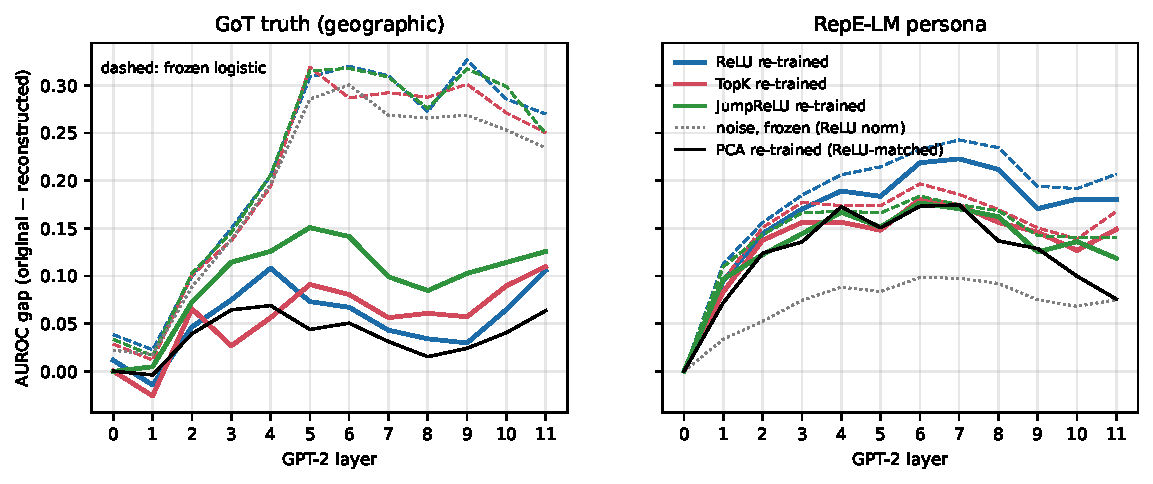
\includegraphics[width=\linewidth]{fig_m2_information}
  \caption{Information preservation by layer (\evlabel{validation}). Dashed: frozen logistic gap; solid: re-trained
  logistic gap; dotted grey: frozen gap under norm-matched noise; black: PCA at the ReLU SAE's error.}
  \label{fig:m2}
\end{figure}

\pending{M5 held-out confirmation; E1 task-level sparsity control; E2 external SAE reference.}
